\section{Assessing the Performance Impact}

\label{sec:predictimprove}
\todo{Adding a picture, maybe similar to Sammati paper}

Fixing false sharing problems can be non-trivial, even with precise information about a particular false sharing problem. Even worse, fixing false sharing problems does not necessarily yield significant speedups. 
\todo{I don't think we show the example here. We evaluate them in the evaluation section. The description here is redundant.} For example, existing tools report a big number of cache invalidations related to false sharing in word\_count or reverse\_index applications, but fixing them brings negligible performance improvement~\cite{Sheriff, Predator}. \todo{This can be moved to related work section.}Zhao et. al. even observed that fixing may even slowdown a program because of excessive memory consumption or the lose of locality~\cite{qinzhao}. Reporting insignificant false sharing instances are not false positives, but that increases manual burden for programmers.

To resolve this problem, \cheetah{} makes the first attempt to quantitatively assess the potential performance gain of fixing a false sharing instance. Thus, programmers can focus on severe problems only, avoiding unnecessary manual effort.
\cheetah{}'s assessment is based on the following observations:
\begin{itemize}
\item {\bf Observation 1:} the sampling is evenly distributed over the whole execution. Based on this, we can  use the results of sampling to represent the whole execution. This idea is widely used by the exiting work like Oprofile and Gprof when they identify the hotspots of function calls and code~\cite{oprofile, DBLP:conf/sigplan/GrahamKM82}.

\item {\bf Observation 2:} PMU hardware provides the latency information (e.g. cycles) of each memory load operation. We also observed that the latency of accessing falsely shared objects is significantly higher than that of normal accesses. 

\end{itemize}
Based on these two observations, {\bf we propose to use the sampled cycles to represent the runtime time of an execution and further predict the performance impact of an falsely-shared object $O$}. The assessment is performed in three steps listed as follows. \todo{There is no need to have the bullets here. Use normal texts to save some space.}

\begin{itemize}
\item \cheetah{} first evaluates the performance impact on accesses on this object $O$, as discussed in Section~\ref{sec:impactobject}. 

\item Then \cheetah{} assesses the performance impact on the related threads by fixing this false sharing problem, which is discussed in Section~\ref{sec:impactthread}. 
 
\item In the end, \cheetah{} assesses the performance impact on the application, seen in Section~\ref{sec:impactapp}. 
\end{itemize}


\subsection{Impact on Accesses of the Object}
\label{sec:impactobject}

To assess the performance impact of fixing a falsely-shared object $O$, \cheetah{} has to collect the following information related to this object $O$:  total cycles of accesses-- $Cycles_O$, total number of accesses--$Accesses_O$, and the average cycles of every memory access after fixing--$AverCycles_{nofs}$.

Based on these numbers, \cheetah{} first predicts the total cycles of all accesses after fixing, noted as $PredictCycles_{O}$ according to EQ.(\ref{eq:predictedcyclesofo}).   
\begin{equation}
\label{eq:predictedcyclesofo}
 PredictCycles_{O} = (AverageCycles_{nofs} * Accesses_O);
\end{equation} 

However, it is impossible to know $AverCycles_{nofs}$ for $O$ after fixing without the actual fix. Thus, {\it \cheetah{} utilizes the average cycles of each access in the serial phases to approximate this}. There is no false sharing in serial phases, thus $AverCycles_{nofs}$ represents the best scenario of fixing an existing false sharing instance. In reality, the cycles of every access after fixing can be larger than the $AverCycles_{nofs}$ here, since fixing false sharing may lead to excessive memory consumption or the lose of locality~\cite{qinzhao}. Thus, our prediction actually provides an upper bound of performance improvement. 
 
\subsection{Impact on Related Threads}
\label{sec:impactthread}

After getting the $PredictCycles_{O}$, \cheetah{} assesses the possible execution time of different threads affected by fixing false sharing of this object $O$. 

\Cheetah{} collects the following information of every thread: the execution time -- $RT_{thread}$, the total number of accesses -- $Accesses_{thread}$, and the total cycles of all memory accesses -- $Cycles_{thread}$.

To collect these numbers, \cheetah{} intercepts the creation of threads by passing a custom function as the start routine. In this custom function, \cheetah{} gets the timestamps of before and after running the thread function, so that it can compute the execution time of a thread ($RT_{thread}$). To gather the number of accesses and cycles of every thread, \cheetah{} makes every thread to respond the signal handler and records the number of accesses and cycles correspondingly  for each sampled memory access, as described in Section~\ref{sec:perfcounter}. 

After the collection, \cheetah{} predicts the new cycles of related thread ($PredictCycles_{thread}$) as the EQ.(\ref{eq:predictedcyclesofthread}). \todo{It's better to simplify the equation denotation. For example, $PredictCycles_{thread}$ can be written as $PC_t$ and you just explain what it means.}
\begin{equation}
\label{eq:predictedcyclesofthread}
 PredictCycles_{thread} = Cycles_{thread} - Cycles_{O} + PredictCycles_{O} 
\end{equation} 
 

Based on this, \cheetah{} assesses the predicted runtime of a thread--- $PredictRT_{thread}$--- as the EQ.(\ref{eq:predictedrtofthread}). In this step, we assume that {\bf the execution time is proportional to the cycles of accesses}: the less of cycles means the less of the execution time.  
\begin{equation}
\label{eq:predictedrtofthread}
 PredictRT_{thread} = (PredictCycles_{thread}/Cycles_{thread}) * RT_{thread} 
\end{equation} 

\subsection{Impact on the Application}
\label{sec:impactapp}

In the end, \cheetah{} assesses how fixing a false sharing instance will change the performance of the application. 

This a very challenging topic. For example, if a thread is not in the critical path, then fixing false sharing problems related to this thread may not have an observed impact on the final performance. The assessment can become even more complicated if nested threads exist inside the application. 

To simplify the prediction and verify our idea, \cheetah{} currently focuses on applications with the normal fork-join model, shown as Figure~\ref{fig:forkjoinmodel}. This model is the most important and widely used model in reality. All applications that we have evaluated in this paper utilizes this fork-join model. 

\begin{figure*}[ht!]
\begin{center}
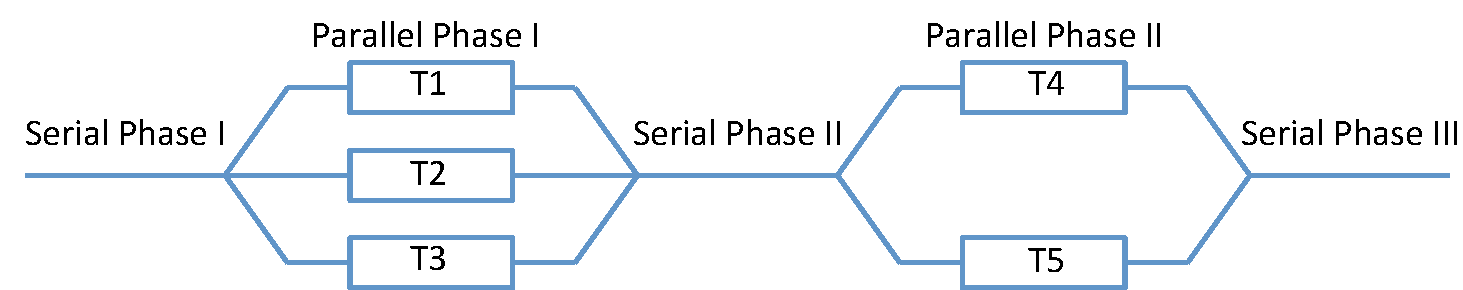
\includegraphics[width=6in]{figure/forkjoin}
\end{center}
\caption{The fork-join model that \Cheetah{} currently focuses on to assess the impact of false sharing instances.   \todo{This figure seems useless in this section. You don't need to show this, as everyone knows what is a fork-join}}
\label{fig:forkjoinmodel}
\end{figure*}

\cheetah{} tracks creations and joins of threads in order to verify whether an application uses the fork-join model or not. \Cheetah{} also collects the execution time (RT) of different serial and parallel phases using RDTSC (ReaD-Time Stamp Counter) available on X86 machines~\cite{rtdsc}: the applications enter the first parallel phase I after the first thread creation; The execution will leave a parallel phase after all children threads are joined successfully. 

After that, \cheetah{} can assess the final performance impact on an application. Based on the predicted execution time of different threads as described in Section~\ref{sec:impactthread}, \cheetah{} recomputes the length of each phase and the total time after fixing: the length of each phase is decided by the thread with the longest execution time, while the total time is equal to the sum of different parallel phases and serial phases. 

\cheetah{} will compute the potential performance improvement based on EQ.(\ref{eq:improvement}), where runtime is denoted by $RT$. We will report the potential performance improvement for every falsely-shared object in the end as Figure~\ref{fig:lr}. Then programmers can focus only on those ones with serious performance impact. We further verify the precision of \cheetah{}'s assessment in Section~\ref{sec:precision}.
\begin{equation}
\label{eq:improvement}
Perf_{improve}= RT_{App} / PredictRT_{App}
\end{equation}

%We will uses an example to show that. For example, there is a false sharing problem that will involved in the $T1$ and $T2$ of Figure~\ref{fig:forkjoinmodel}, but not other threads.  We will assess the possible runtime of $PredictRT_{T1}$ and $PredictRT_{T2}$. Then we checked that whether these predicted runtime will affect the runtime of parallel phase I by checking whether these two runtime are less than the runtime of $T3$ at first. If it won't, then fixing the false sharing problem won't affect the final performance. Otherwise, we have to recompute the length of parallel phase I, while the length of other phases will keep the same. By doing that, we will get a new runtime for the application. Using the EQ.(\ref{eq:improvement}), we can compute the potential performance improvement of this application by fixing the false sharing problems related to the thread $T1$ and $T2$. 









